% Comandos especiais

\newcommand{\matriz}[1]{%
  \begin{equation}\begin{bmatrix}
    #1
  \end{bmatrix}\end{equation}
}

\newcommand{\esquema}{%
  \begin{center}
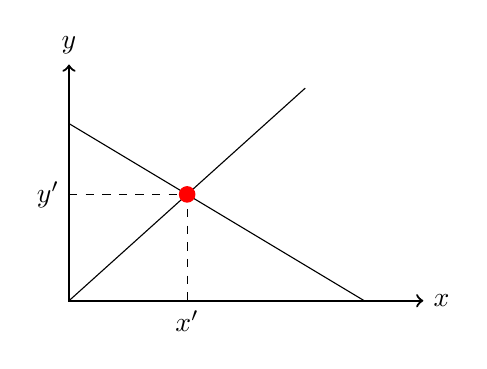
\begin{tikzpicture}[scale=1.5]
    % Draw axes
    \draw [<->,thick] (0,2) node (yaxis) [above] {$y$}
        |- (3,0) node (xaxis) [right] {$x$};
    % Draw two intersecting lines
    \draw (0,0) coordinate (a_1) -- (2,1.8) coordinate (a_2);
    \draw (0,1.5) coordinate (b_1) -- (2.5,0) coordinate (b_2);
    % Calculate the intersection of the lines a_1 -- a_2 and b_1 -- b_2
    % and store the coordinate in c.
    \coordinate (c) at (intersection of a_1--a_2 and b_1--b_2);
    % Draw lines indicating intersection with y and x axis. Here we use
    % the perpendicular coordinate system
    \draw[dashed] (yaxis |- c) node[left] {$y'$}
        -| (xaxis -| c) node[below] {$x'$};
    % Draw a dot to indicate intersection point
    \fill[red] (c) circle (2pt);
\end{tikzpicture}
\end{center}
}

% Conteúdo

\newcommand\titulo{Título}
\newcommand\autor{Autor}
\newcommand\organizador{Organizador}
\newcommand\tradutor{Tradutor}
\newcommand\cidade{São Paulo}
\newcommand\ano{2013}
\newcommand\direitos{Hedra}
\newcommand\introducao{\chapter{Introdução}
                          \esquema\lipsum[1-4]}
\newcommand\texto{\chapter{Texto 1}
    \matriz{12 & 12 & 12\\ 
    34 & 2 & 12\\
    12 & 12 & 12\\}
                          \lipsum[2]
    \matriz{2 & 22 \\
            34 & 34}
                  \chapter{Texto 2}
                          \lipsum[42-53]}


